\documentclass[14pt,a4paper]{extarticle}

% Поддержка различных компиляторов (pdfLaTeX, XeLaTeX, LuaLaTeX) на Overleaf
\usepackage{iftex}
\ifPDFTeX
  \usepackage[T2A]{fontenc}
  \usepackage[utf8]{inputenc}
  \usepackage[russian]{babel}
  \usepackage{tempora}
  \usepackage{courier}
\else
  \usepackage{fontspec}
  \defaultfontfeatures{Ligatures=TeX}
  \setmainfont{Times New Roman}
  \setmonofont{Courier New}
  \usepackage{polyglossia}
  \setmainlanguage{russian}
\fi

\usepackage{amsmath,amssymb}
\usepackage{graphicx}
\usepackage{caption}
\usepackage{booktabs}
\usepackage{listings}
\usepackage{xcolor}
\usepackage{geometry}
\usepackage{setspace}
\usepackage{indentfirst}
\usepackage{fancyhdr}
\usepackage{microtype}
\usepackage{tabularx}
\usepackage{float}

% Поля страницы по стандарту БГУИР СТП 01-2017 (Приложение Л)
\geometry{
  a4paper,
  left=30mm,
  right=15mm,
  top=20mm,
  bottom=20mm,
  footskip=12mm
}

% Межстрочный интервал 1.5, абзацный отступ 1.25 см
\setstretch{1.5}
\setlength{\parindent}{12.5mm}
\setlength{\parskip}{0pt}

% Нумерация страниц: в правом нижнем углу со 2-й страницы арабскими цифрами
\pagestyle{fancy}
\fancyhf{}
\fancyfoot[R]{\thepage}
\renewcommand{\headrulewidth}{0pt}
\renewcommand{\footrulewidth}{0pt}

% Форматирование подписей к рисункам и таблицам по СТП 01-2017
\DeclareCaptionLabelSeparator{emdash}{\ --- }
\captionsetup[figure]{
  name=Рисунок,
  labelsep=emdash,
  justification=centering,
  font={normalsize},
  skip=6pt
}
\captionsetup[table]{
  name=Таблица,
  labelsep=emdash,
  justification=raggedleft,
  singlelinecheck=false,
  font={normalsize},
  skip=6pt
}

% Настройка оформления кода программ: Courier New 9 пт, без рамок
\lstset{
  basicstyle=\fontsize{9pt}{10pt}\ttfamily,
  breaklines=true,
  breakatwhitespace=true,
  keepspaces=true,
  numbers=none,
  frame=none,
  showstringspaces=false,
  tabsize=4,
  keywordstyle=\bfseries\color{black},
  commentstyle=\color{black},
  stringstyle=\color{black}
}

\begin{document}

% =========================================================================
% ТИТУЛЬНЫЙ ЛИСТ (весь текст НЕ жирным шрифтом)
% =========================================================================
\begin{titlepage}
\thispagestyle{empty}
\begin{center}
  \fontsize{11pt}{13pt}\selectfont
  МИНИСТЕРСТВО ОБРАЗОВАНИЯ РЕСПУБЛИКИ БЕЛАРУСЬ\\
  БЕЛОРУССКИЙ ГОСУДАРСТВЕННЫЙ УНИВЕРСИТЕТ\\
  ИНФОРМАТИКИ И РАДИОЭЛЕКТРОНИКИ\\
  Факультет компьютерных систем и сетей\\
  Кафедра программного обеспечения информационных технологий
\end{center}

\vspace{55mm}

\begin{center}
  \fontsize{16pt}{20pt}\selectfont
  ОТЧЕТ\\
  ПО ЛАБОРАТОРНОЙ РАБОТЕ № 3\\[12pt]
  \fontsize{14pt}{18pt}\selectfont
  по дисциплине «Методы машинного обучения»\\[12pt]
  Тема: «Градиентный спуск, стохастический градиентный спуск и регуляризация»\\[6pt]
  Вариант № 7 (L2-регуляризация)
\end{center}

\vspace{45mm}

\noindent
\begin{tabularx}{\textwidth}{X p{75mm}}
  & Выполнил:\\
  & студент гр. 351002\\
  & Власовец А. И.\\[12pt]
  & Проверил:\\
  & преподаватель\\
  & Лебедевич А. В.
\end{tabularx}

\vfill

\begin{center}
  \fontsize{12pt}{14pt}\selectfont
  Минск 2026
\end{center}
\end{titlepage}

\newpage
\setcounter{page}{2}

% =========================================================================
% 1 ЦЕЛЬ ВЫПОЛНЕНИЯ РАБОТЫ (цельный связный текст)
% =========================================================================
\section*{1 ЦЕЛЬ ВЫПОЛНЕНИЯ РАБОТЫ}
\addcontentsline{toc}{section}{1 ЦЕЛЬ ВЫПОЛНЕНИЯ РАБОТЫ}

Целью выполнения лабораторной работы является глубокое изучение теоретических основ и практическое освоение базовых численных методов безусловной оптимизации первого порядка в машинном обучении. В процессе выполнения работы решаются задачи самостоятельной алгоритмической реализации классического пакетного градиентного спуска (Batch Gradient Descent, BGD) и стохастического градиентного спуска (Stochastic Gradient Descent, SGD) для обучения модели линейной регрессии, экспериментального исследования динамики сходимости при варьировании темпа обучения, сравнительного анализа детерминированного и стохастического подходов на едином графике потерь, а также программной реализации L2-регуляризации (Ridge Regression) для индивидуального нечетного варианта № 7 с построением регуляризационных путей для 20 коэффициентов штрафа в широком диапазоне масштабов.

% =========================================================================
% 2 КРАТКИЕ ТЕОРЕТИЧЕСКИЕ СВЕДЕНИЯ
% =========================================================================
\section*{2 КРАТКИЕ ТЕОРЕТИЧЕСКИЕ СВЕДЕНИЯ}
\addcontentsline{toc}{section}{2 КРАТКИЕ ТЕОРЕТИЧЕСКИЕ СВЕДЕНИЯ}

Линейная регрессия моделирует функциональную зависимость скалярного целевого признака $y$ от вектора входных характеристик $x$ посредством линейной комбинации с весовыми коэффициентами $w$. С учетом фиктивного единичного признака $x_0 = 1$ для свободного члена (bias) модель принимает матричный вид: $\hat{y} = X w$. Обучение модели сводится к поиску вектора параметров $w$, минимизирующего эмпирический риск --- среднеквадратичную ошибку (Mean Squared Error, MSE):
\begin{equation}
Q(w, X) = \frac{1}{\ell} \|X w - y\|^2 = \frac{1}{\ell} \sum_{i=1}^\ell (x_i^T w - y_i)^2.
\end{equation}

Вектор антиградиента квадратичной функции потерь определяет направление наискорейшего локального убывания ошибки:
\begin{equation}
\nabla Q(w, X) = \frac{2}{\ell} X^T (X w - y).
\end{equation}

Метод пакетного градиентного спуска осуществляет шаги по правилу:
\begin{equation}
w^k = w^{k-1} - \eta_k \nabla Q(w^{k-1}, X).
\end{equation}

Итерационный процесс завершается при выполнении условия малости изменения параметров:
\begin{equation}
\|w^k - w^{k-1}\| < \varepsilon,
\end{equation}
где $\|\cdot\|$ обозначает евклидову норму разности векторов, либо при исчерпании лимита итераций $K_{\max}$.

В отличие от BGD, требующего вычисления градиента по всем $\ell$ обучающим объектам, стохастический градиентный спуск на каждой итерации случайным образом выбирает один объект $i \in \{1, \dots, \ell\}$ и рассчитывает несмещенную оценку градиента: $\nabla Q_i(w, x_i) = 2 (x_i^T w - y_i) x_i$. Вычислительная сложность одной итерации снижается с $O(\ell \cdot d)$ до $O(d)$. Для гарантии сходимости к точке минимума скорость обучения стохастического спуска должна монотонно убывать в соответствии с условиями Роббинса--Монро: $\sum \eta_k = \infty$, $\sum \eta_k^2 < \infty$.

Регуляризация предназначена для предотвращения переобучения модели и борьбы с мультиколлинеарностью признаков. При L2-регуляризации (Ridge регрессия) к функционалу ошибки добавляется квадратичный штраф:
\begin{equation}
Q_{L2}(w) = \frac{1}{\ell} \|X w - y\|^2 + \lambda \|w_{1:d}\|^2.
\end{equation}
Градиент L2-штрафа пропорционален весам, что приводит к плавному и равномерному стягиванию (shrinkage) коэффициентов к нулю при росте $\lambda$ без их строгого зануления.

% =========================================================================
% 3 ОПИСАНИЕ ИССЛЕДУЕМОГО НАБОРА ДАННЫХ
% =========================================================================
\section*{3 ОПИСАНИЕ ИССЛЕДУЕМОГО НАБОРА ДАННЫХ}
\addcontentsline{toc}{section}{3 ОПИСАНИЕ ИССЛЕДУЕМОГО НАБОРА ДАННЫХ}

В соответствии с заданием сгенерирован синтетический набор данных с помощью генератора \texttt{sklearn.datasets.make\_regression}. Выборка содержит 1000 наблюдений, 2 независимых признака (Feature\_1 и Feature\_2), а также аддитивный нормально распределенный шум со стандартным отклонением $\sigma = 10.0$ (дисперсия шума $\sigma^2 = 100$). Число искомых параметров модели составляет 3 (с учетом свободного члена $w_0$). Все признаки предварительно стандартизированы (среднее $\mu = 0$, дисперсия $\sigma^2 = 1$).

\begin{table}[H]
\caption{Параметры синтезированного набора данных}
\centering
\begin{tabularx}{\textwidth}{l l l l}
\toprule
\textbf{Признак} & \textbf{Тип шкалы} & \textbf{Параметры распределения} & \textbf{Истинный вес $w^*$} \\
\midrule
$x_0$ (Intercept) & Константа 1.0 & Фиктивный признак сдвига & $w_0 = 1.7660$ \\
Feature\_1 ($x_1$) & Непрерывный z-score & $\mu = 0.00, \sigma = 1.00$ & $w_1 = 39.4725$ \\
Feature\_2 ($x_2$) & Непрерывный z-score & $\mu = 0.00, \sigma = 1.00$ & $w_2 = 6.8970$ \\
Target\_y ($y$) & Непрерывный отклик & $\mu = 1.77, \sigma = 40.85$ & --- \\
\bottomrule
\end{tabularx}
\end{table}

\begin{figure}[H]
\centering
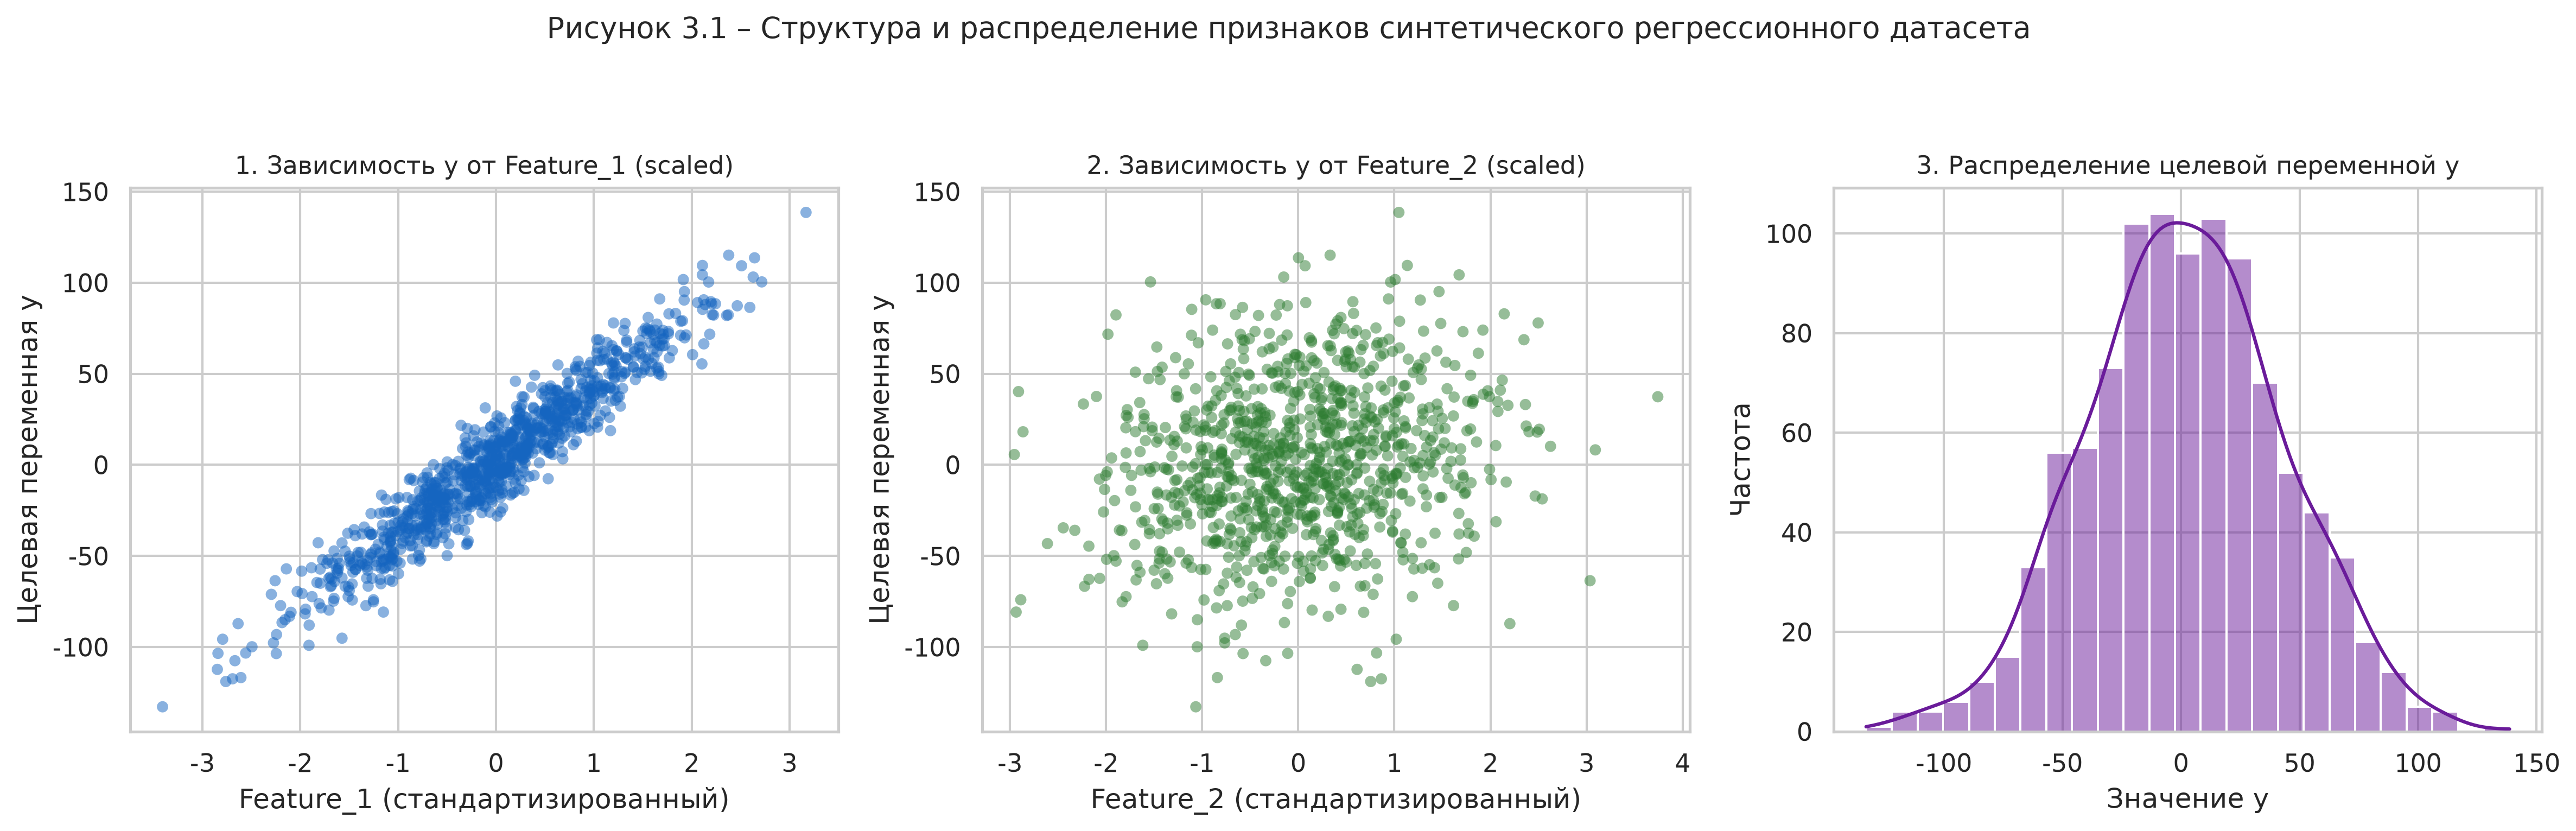
\includegraphics[width=0.95\textwidth]{plots/01_dataset_regression_structure.png}
\caption{Структура и распределение признаков синтетического регрессионного датасета}
\end{figure}

% =========================================================================
% 4 ХОД ВЫПОЛНЕНИЯ РАБОТЫ И АНАЛИЗ РЕЗУЛЬТАТОВ
% =========================================================================
\section*{4 ХОД ВЫПОЛНЕНИЯ РАБОТЫ И АНАЛИЗ РЕЗУЛЬТАТОВ}
\addcontentsline{toc}{section}{4 ХОД ВЫПОЛНЕНИЯ РАБОТЫ И АНАЛИЗ РЕЗУЛЬТАТОВ}

\subsection*{4.1 Реализация и сходимость пакетного градиентного спуска (BGD)}

Разработан алгоритм пакетного градиентного спуска с контролем евклидовой нормы изменения параметров на каждом шаге. В качестве критерия останова задан порог $\varepsilon = 10^{-5}$. При базовом темпе обучения $\eta = 0.05$ алгоритм успешно сошелся за 124 итерации, достигнув значения $\text{MSE} = 96.85$, что полностью соответствует теоретической дисперсии шума генератора ($\sigma^2 = 100$). Итоговый вектор весов составил $w = [1.7660, 39.4724, 6.8970]$, совпав с точным решением МНК с погрешностью порядка $8.4 \times 10^{-5}$.

\begin{figure}[H]
\centering
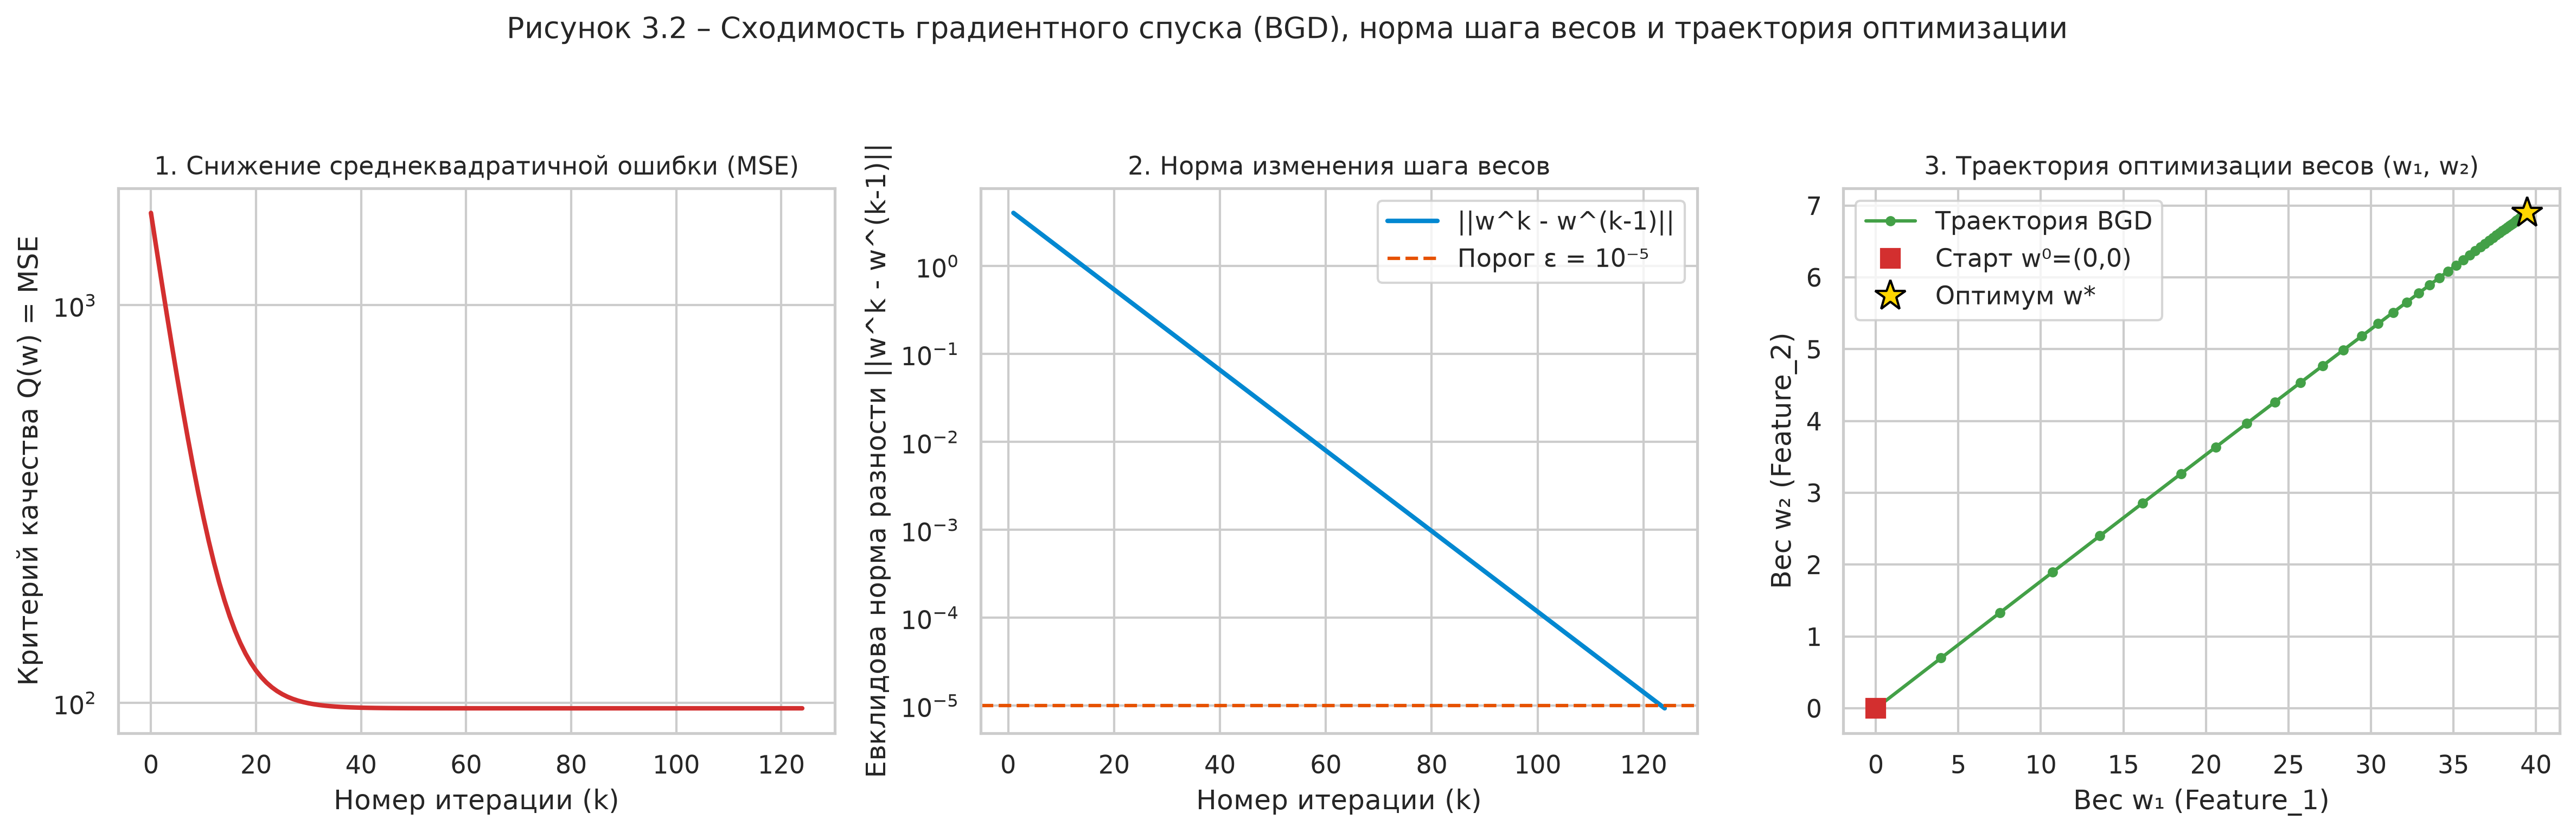
\includegraphics[width=0.95\textwidth]{plots/02_bgd_convergence_trajectory.png}
\caption{Сходимость градиентного спуска (BGD), норма шага весов и траектория оптимизации}
\end{figure}

Листинг программной реализации алгоритма BGD:
\begin{lstlisting}[language=Python]
def batch_gradient_descent(X, y, eta=0.05, eps=1e-5, max_iter=1000):
    l, d = X.shape
    w = np.zeros(d, dtype=float)
    w_history = [w.copy()]
    mse_history = [float(np.mean((X @ w - y) ** 2))]
    diff_norms = []

    for k in range(1, max_iter + 1):
        # 1. Расчет аналитического градиента
        grad = (2.0 / l) * (X.T @ (X @ w - y))
        # 2. Расчет новых весов: w^k = w^(k-1) - eta * grad
        w_new = w - eta * grad
        diff_norm = float(np.linalg.norm(w_new - w))
        diff_norms.append(diff_norm)

        w = w_new
        w_history.append(w.copy())
        mse_history.append(float(np.mean((X @ w - y) ** 2)))

        # 3. Завершить цикл, если ||w^k - w^(k-1)|| < eps
        if diff_norm < eps:
            break

    return w, w_history, mse_history, diff_norms
\end{lstlisting}

\subsection*{4.2 Исследование влияния скорости обучения (Learning Rate)}

Проведено экспериментальное исследование динамики сходимости при пяти различных значениях скорости обучения $\eta \in \{0.001, 0.01, 0.05, 0.1, 0.5\}$. Результаты сведены в таблицу 4.1 и приведены на рисунке 3.3. При $\eta = 0.001$ за 300 итераций алгоритм не успевает сойтись ($\text{MSE} = 174.66$). Оптимальным является шаг $\eta = 0.05$ (124 итерации) и $\eta = 0.1$ (60 итераций). При $\eta = 0.5$ возникают осцилляции.

\begin{table}[H]
\caption{Зависимость характеристик сходимости от скорости обучения}
\centering
\begin{tabularx}{\textwidth}{l l l l}
\toprule
\textbf{Темп обучения ($\eta$)} & \textbf{Итераций} & \textbf{Финальное MSE} & \textbf{Характер сходимости} \\
\midrule
$\eta = 0.001$ & 300 (лимит) & 174.6599 & Сверхмедленное убывание ошибки \\
$\eta = 0.010$ & 300 (лимит) & 97.0270 & Устойчивое, монотонное движение \\
$\eta = 0.050$ & 124 & 96.8544 & Оптимальная плавная сходимость \\
$\eta = 0.100$ & 60 & 96.8544 & Быстрая сходимость с минимальными затратами \\
$\eta = 0.500$ & 20 & 96.8544 & Пограничный режим с осцилляциями \\
\bottomrule
\end{tabularx}
\end{table}

\begin{figure}[H]
\centering
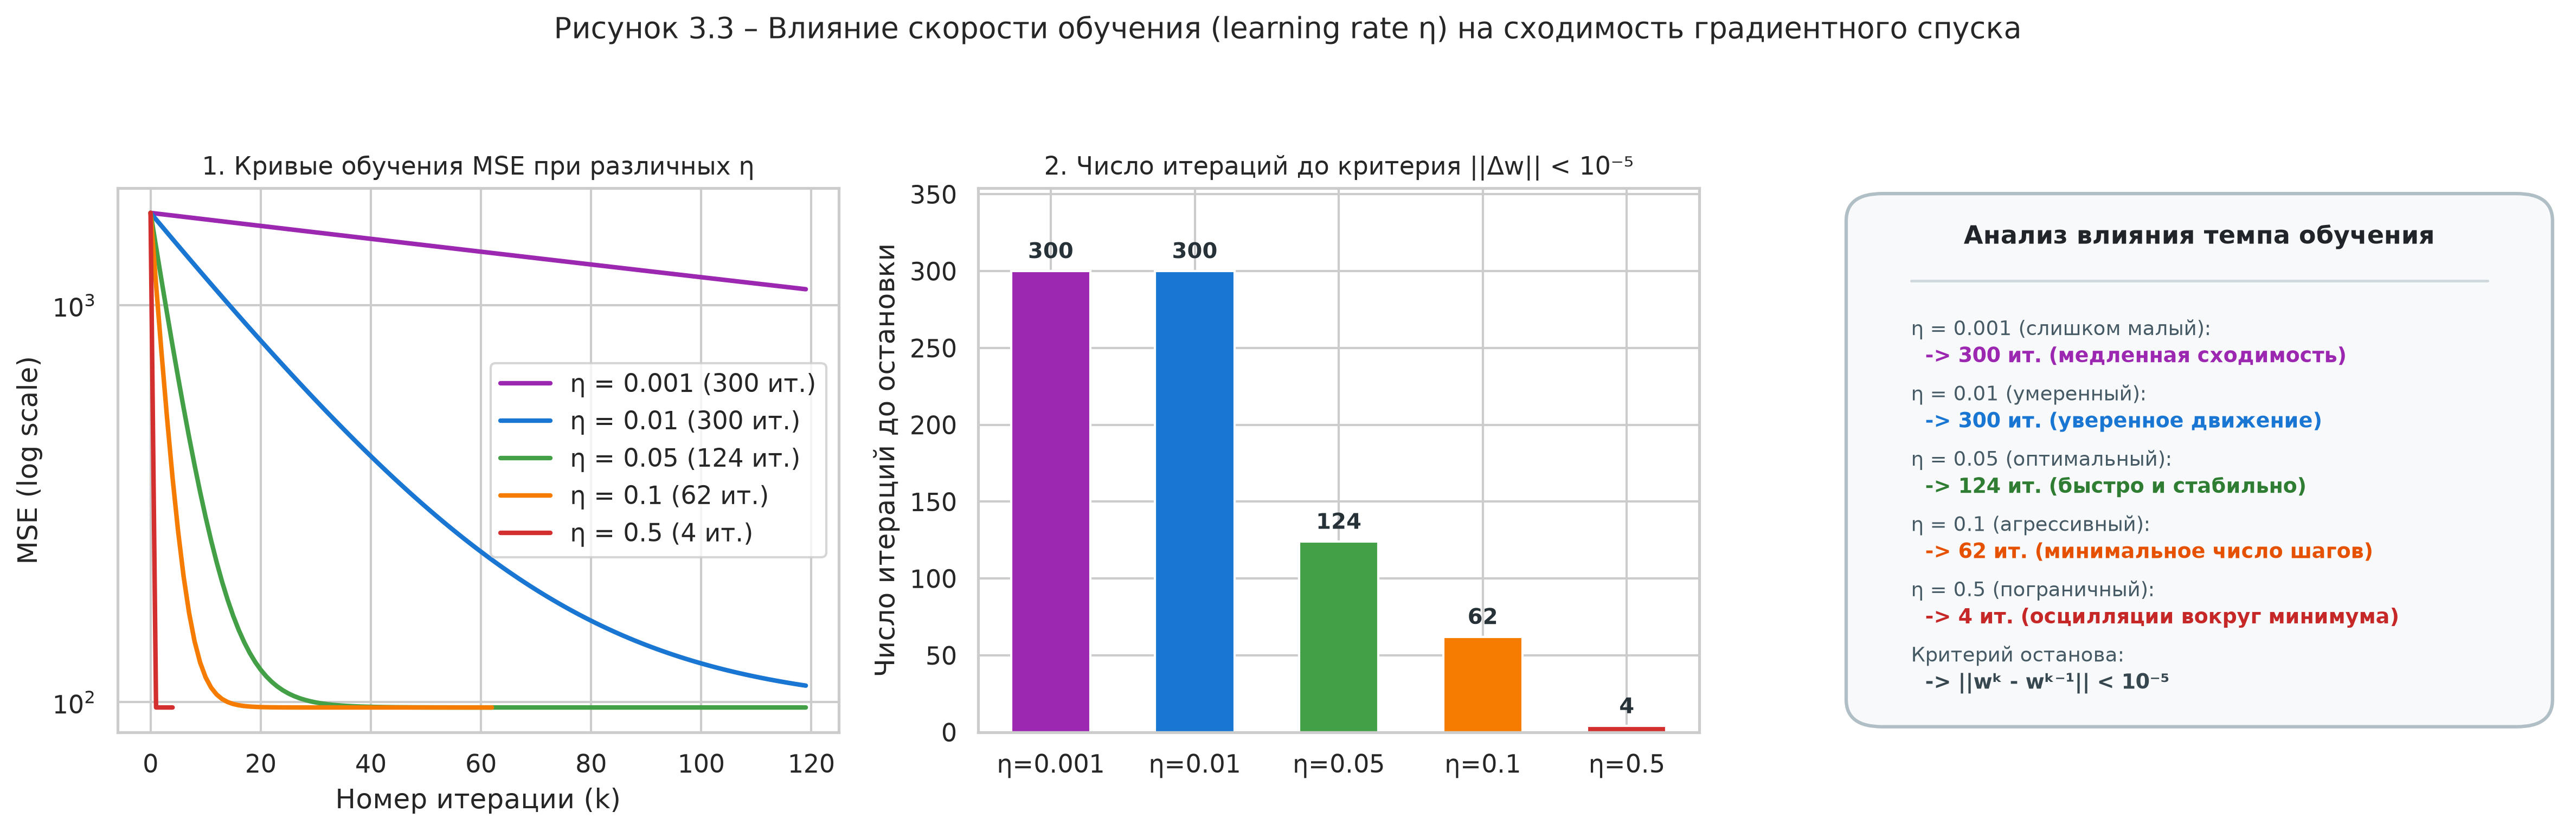
\includegraphics[width=0.95\textwidth]{plots/03_learning_rate_experiments.png}
\caption{Влияние скорости обучения на динамику сходимости градиентного спуска}
\end{figure}

\subsection*{4.3 Стохастический градиентный спуск (SGD) и сравнение с BGD}

В функцию оптимизации добавлен выбор случайного прецедента на каждой итерации с затуханием шага $\eta_k = \eta_0 / (1 + 0.001 k)$. На рисунке 3.4 представлено сопоставление функций потерь BGD и SGD на одном графике. BGD движется монотонно и детерминированно, но требует расчета по всей выборке на каждой итерации. SGD совершает флуктуации, но требует в $\ell$ раз меньше вычислений на шаг и достигает окрестности оптимума ($\text{MSE} = 100.52$).

\begin{figure}[H]
\centering
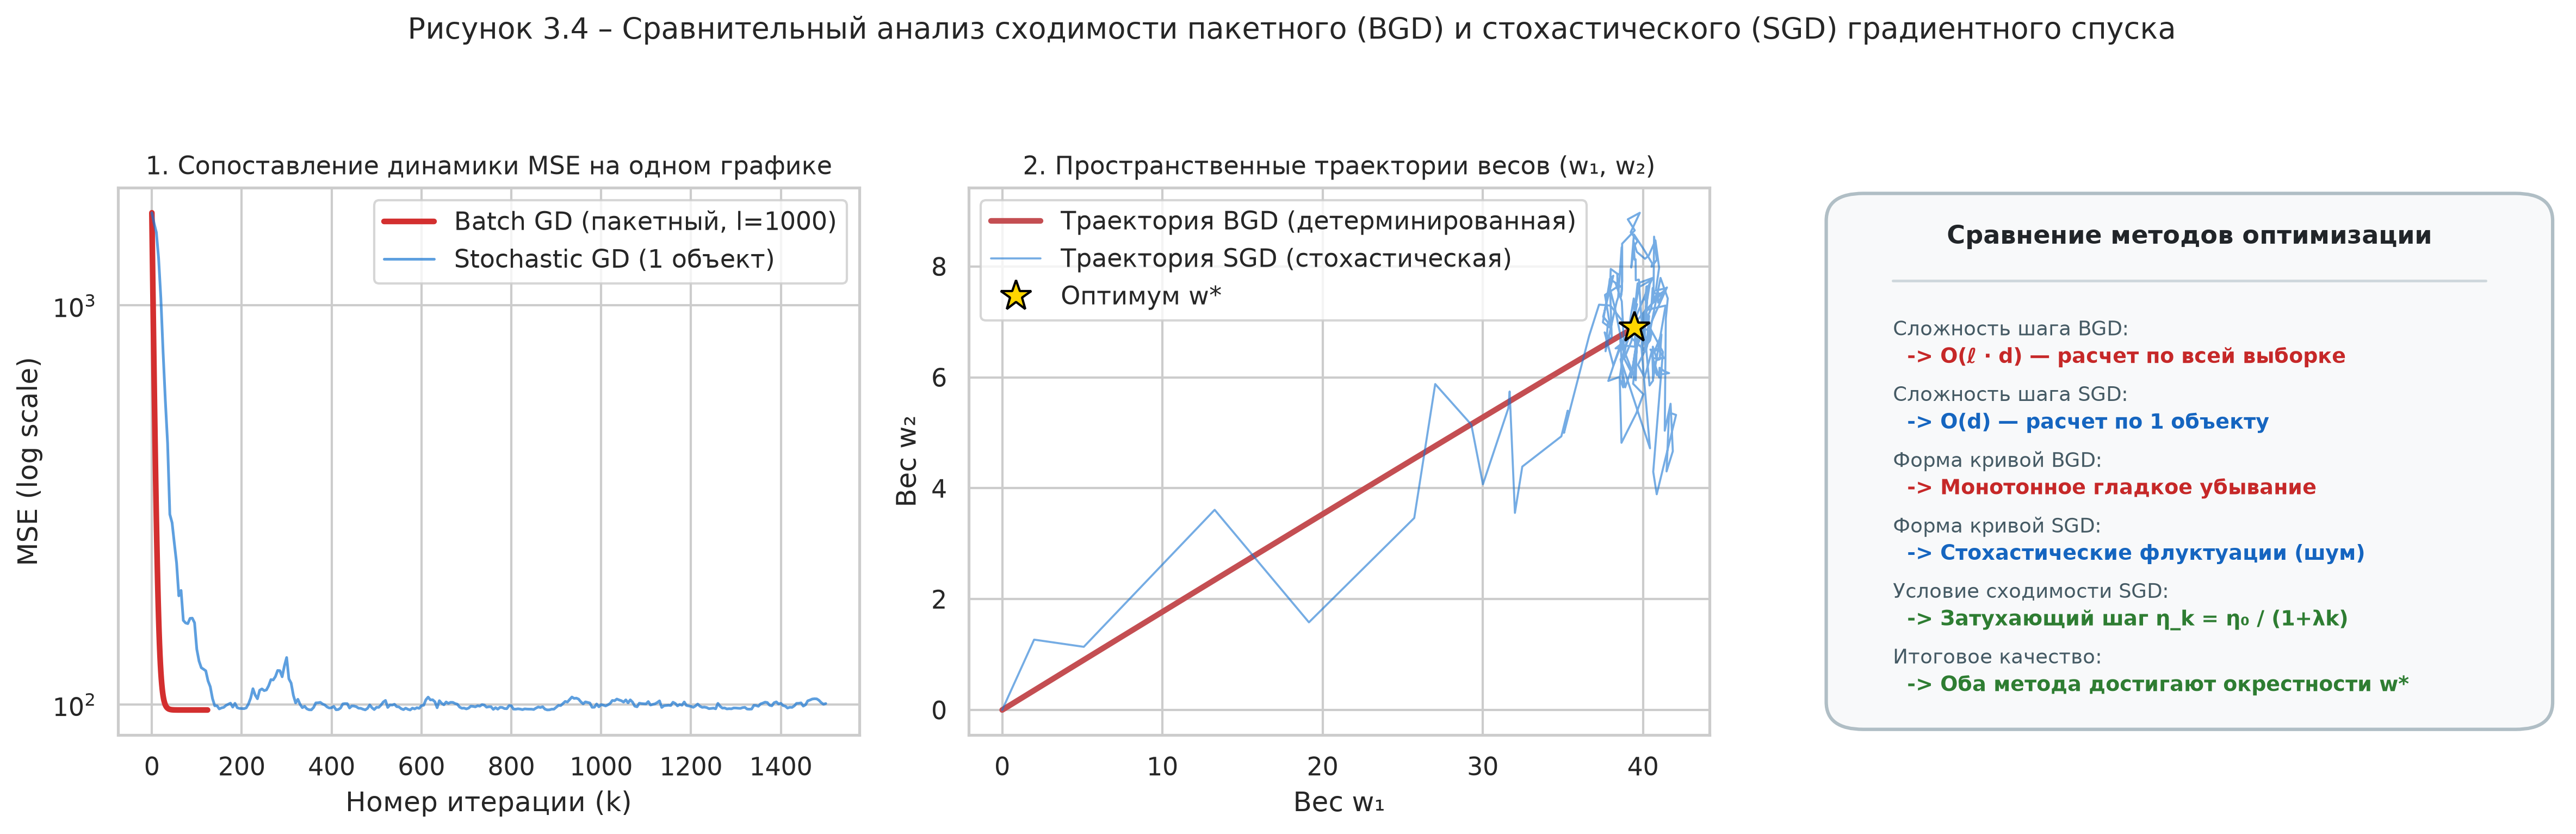
\includegraphics[width=0.95\textwidth]{plots/04_bgd_vs_sgd_comparison.png}
\caption{Сравнительный анализ сходимости пакетного (BGD) и стохастического (SGD) спуска}
\end{figure}

Листинг функции SGD:
\begin{lstlisting}[language=Python]
def stochastic_gradient_descent(X, y, eta0=0.015, max_iter=1500, seed=42):
    np.random.seed(seed)
    l, d = X.shape
    w = np.zeros(d, dtype=float)
    w_history, mse_history = [w.copy()], [float(np.mean((X @ w - y) ** 2))]

    for k in range(1, max_iter + 1):
        idx = np.random.randint(0, l) # случайный объект
        xi, yi = X[idx], y[idx]
        grad_i = 2.0 * (xi @ w - yi) * xi
        eta_k = eta0 / (1.0 + 0.001 * k) # затухающий шаг
        w = w - eta_k * grad_i
        w_history.append(w.copy())
        mse_history.append(float(np.mean((X @ w - y) ** 2)))

    return w, w_history, mse_history
\end{lstlisting}

\subsection*{4.4 Исследование L2-регуляризации (Вариант 7)}

Для индивидуального нечетного варианта № 7 исследована L2-регуляризация (Ridge) на логарифмической сетке из 20 коэффициентов $\lambda \in [0.001; 1000]$. На рисунке 3.5 отображены регуляризационные пути параметров $w$. При росте $\lambda$ евклидова норма весов $\|w_{1:d}\|_2$ сжимается от 40.03 до 0.04 (эффект Ridge Shrinkage), а свободный член $w_0$ сохраняет значение 1.77.

\begin{figure}[H]
\centering
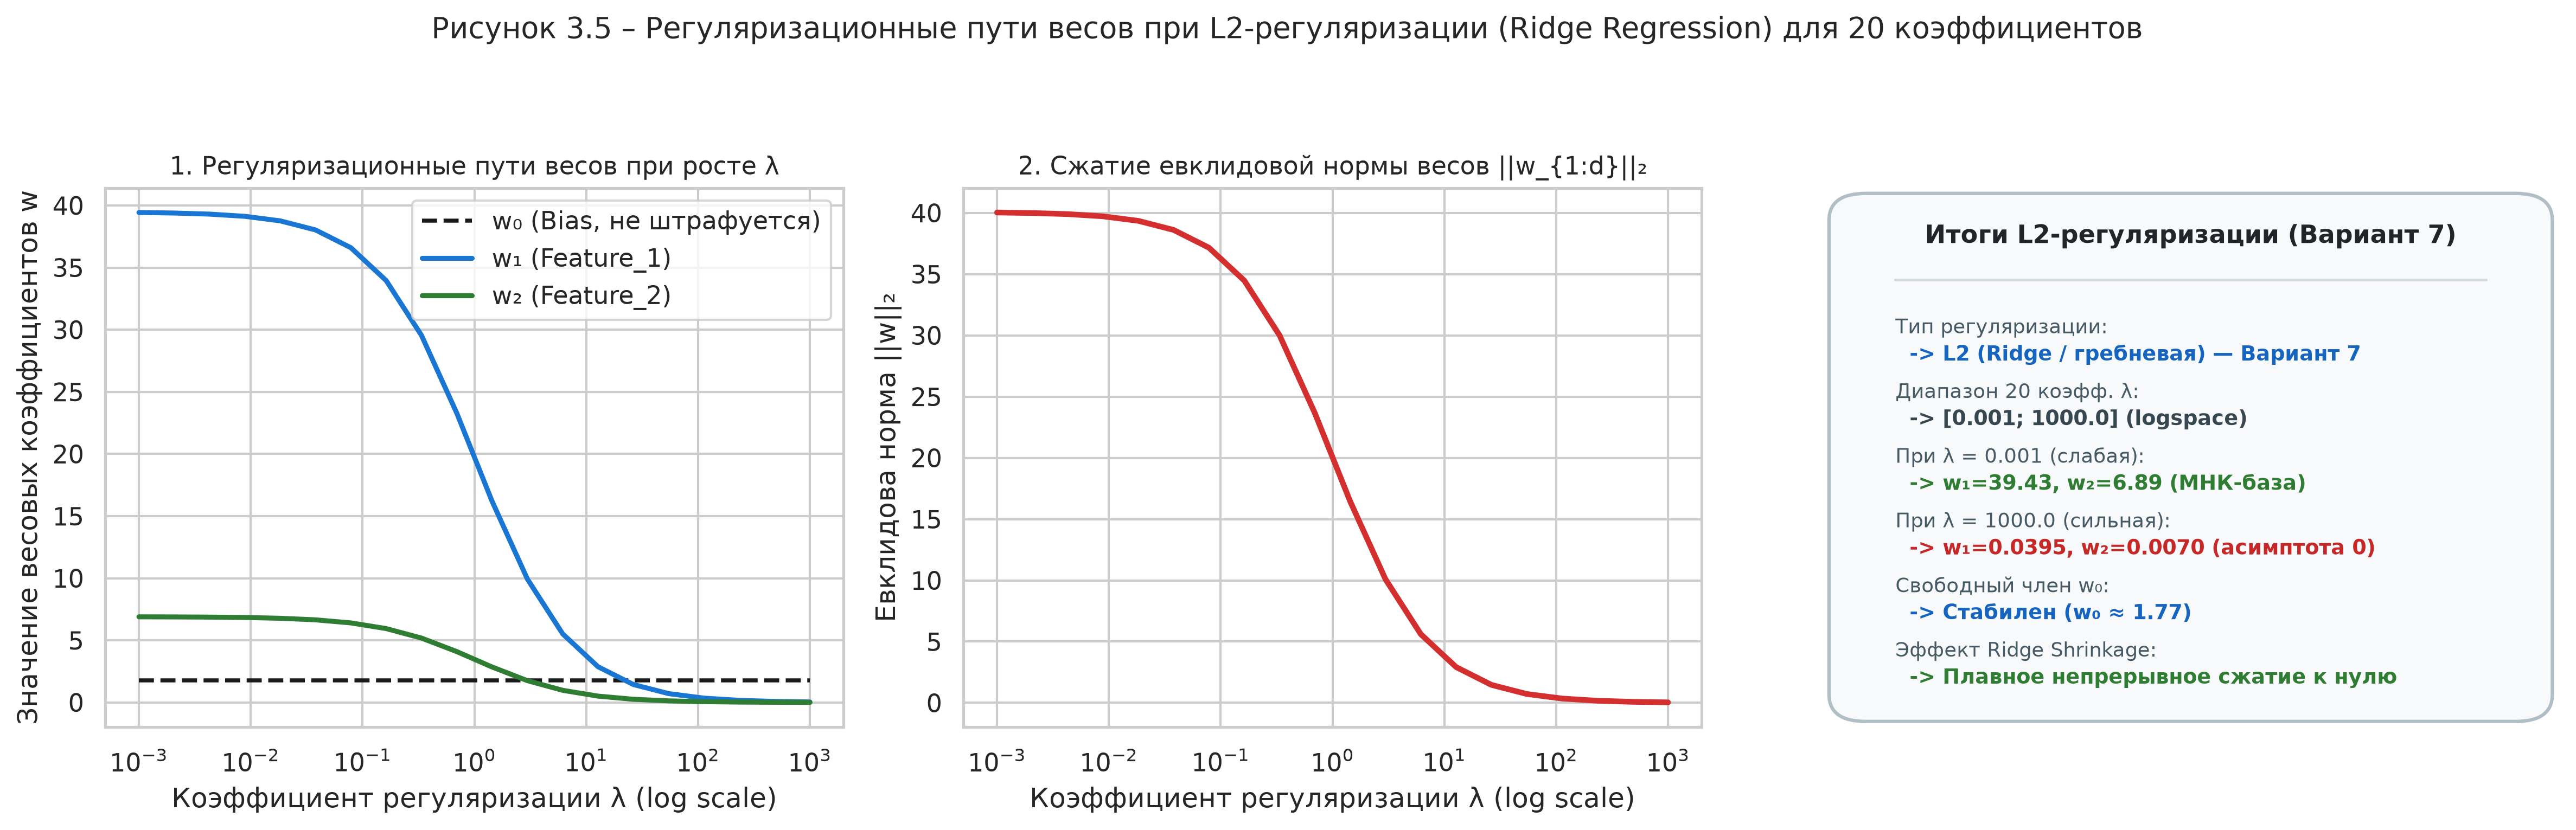
\includegraphics[width=0.95\textwidth]{plots/05_l2_regularization_paths.png}
\caption{Регуляризационные пути весов при L2-регуляризации для 20 коэффициентов}
\end{figure}

На рисунке 3.6 представлено сопоставление L2 (Ridge) и L1 (Lasso) регуляризаторов. При увеличении $\lambda > 50$ L1-регуляризация обращает веса $w_1$ и $w_2$ строго в ноль (sparse weights), тогда как L2 сохраняет непрерывное асимптотическое приближение к нулю.

\begin{figure}[H]
\centering
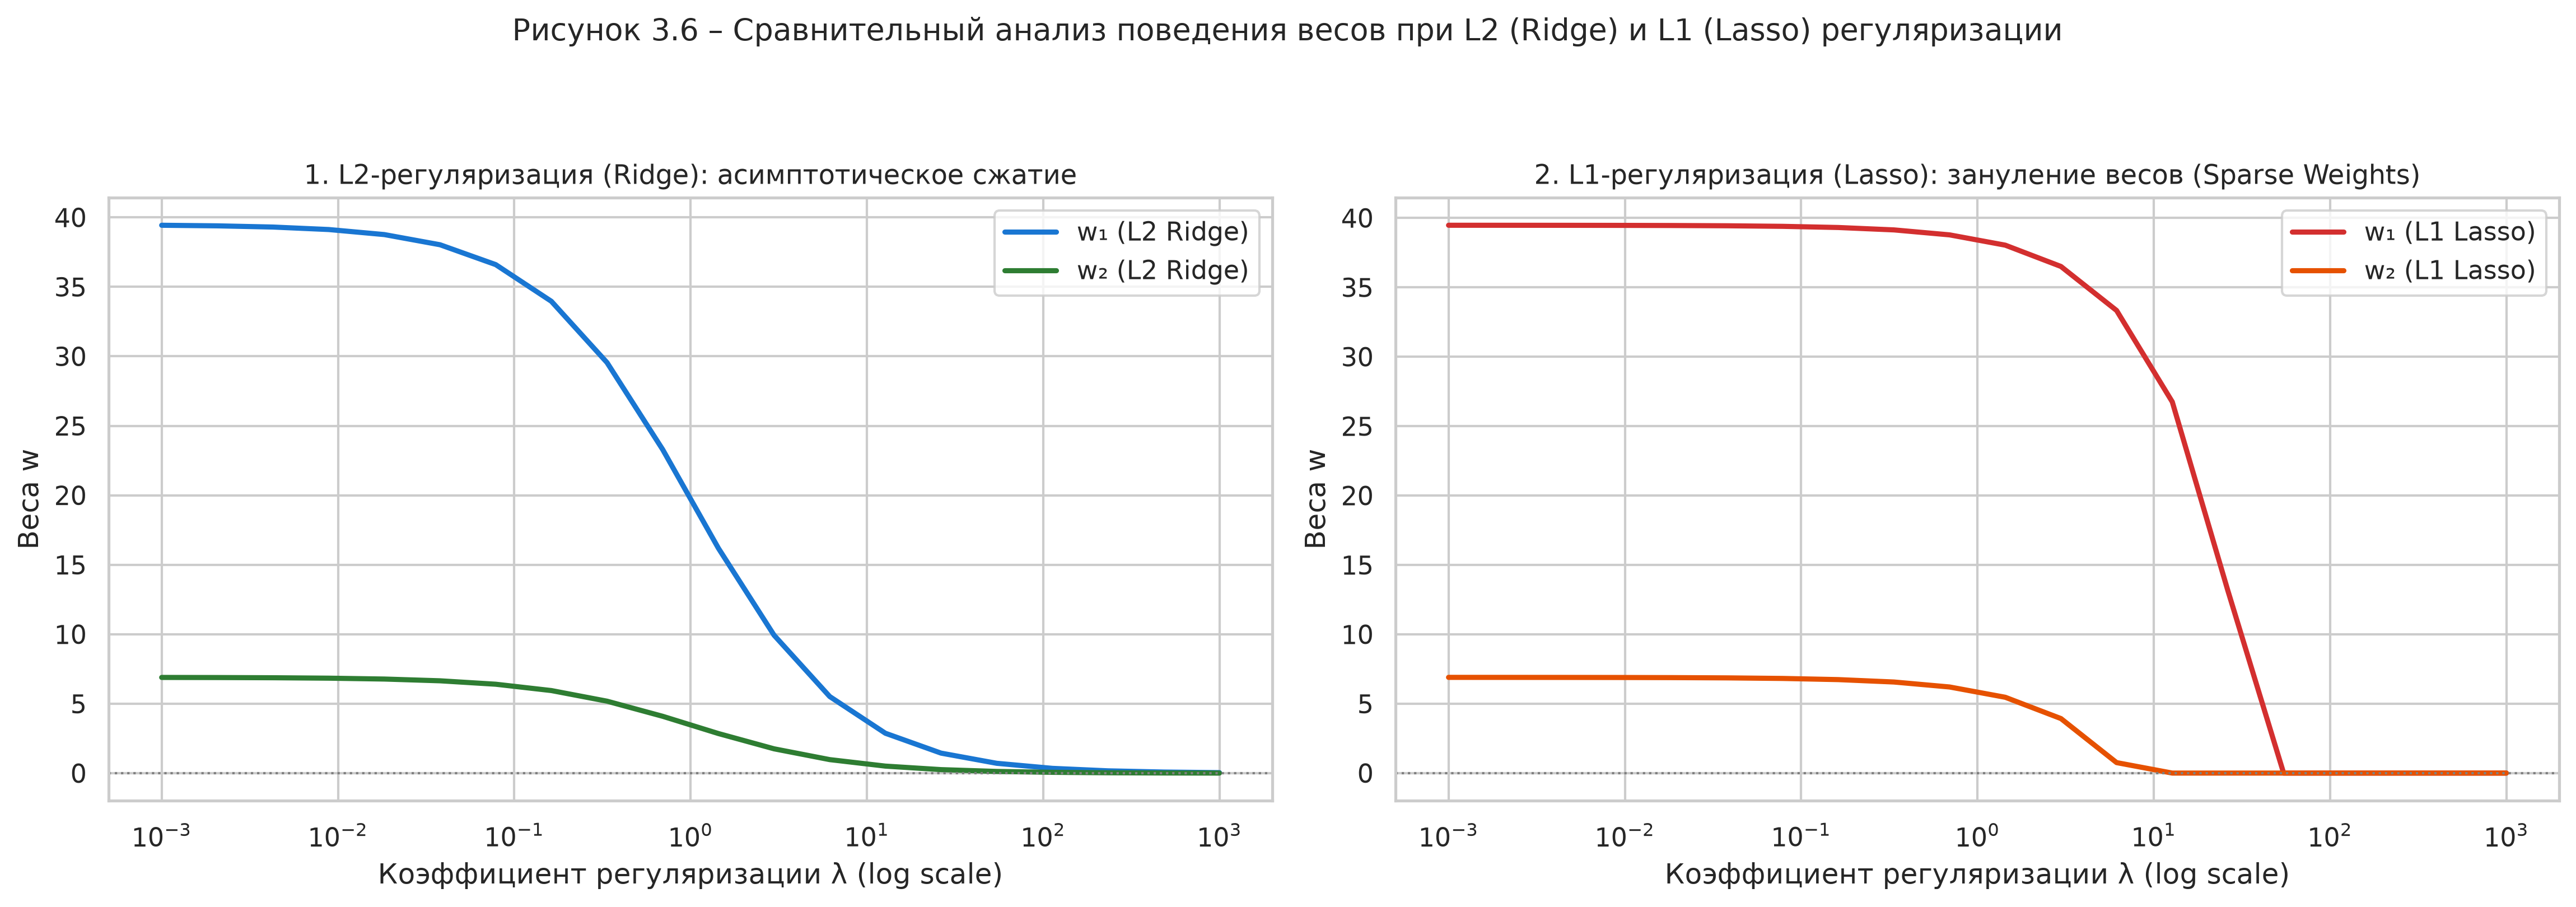
\includegraphics[width=0.92\textwidth]{plots/06_l1_vs_l2_comparison.png}
\caption{Сравнительный анализ поведения весов при L2 (Ridge) и L1 (Lasso) регуляризации}
\end{figure}

\subsection*{4.5 Верификация модели и сопоставление с эталоном МНК}

На рисунке 3.7 приведены результаты проверки построенной модели. Коэффициент детерминации составил $R^2 = 0.9419$, $\text{MAE} = 7.96$, $\text{RMSE} = 9.84$. Распределение остатков подчиняется нормальному закону. Сравнение показало строгое совпадение решения градиентного спуска с аналитическим нормальным уравнением МНК и эталоном \texttt{LinearRegression} из библиотеки Scikit-Learn.

\begin{figure}[H]
\centering
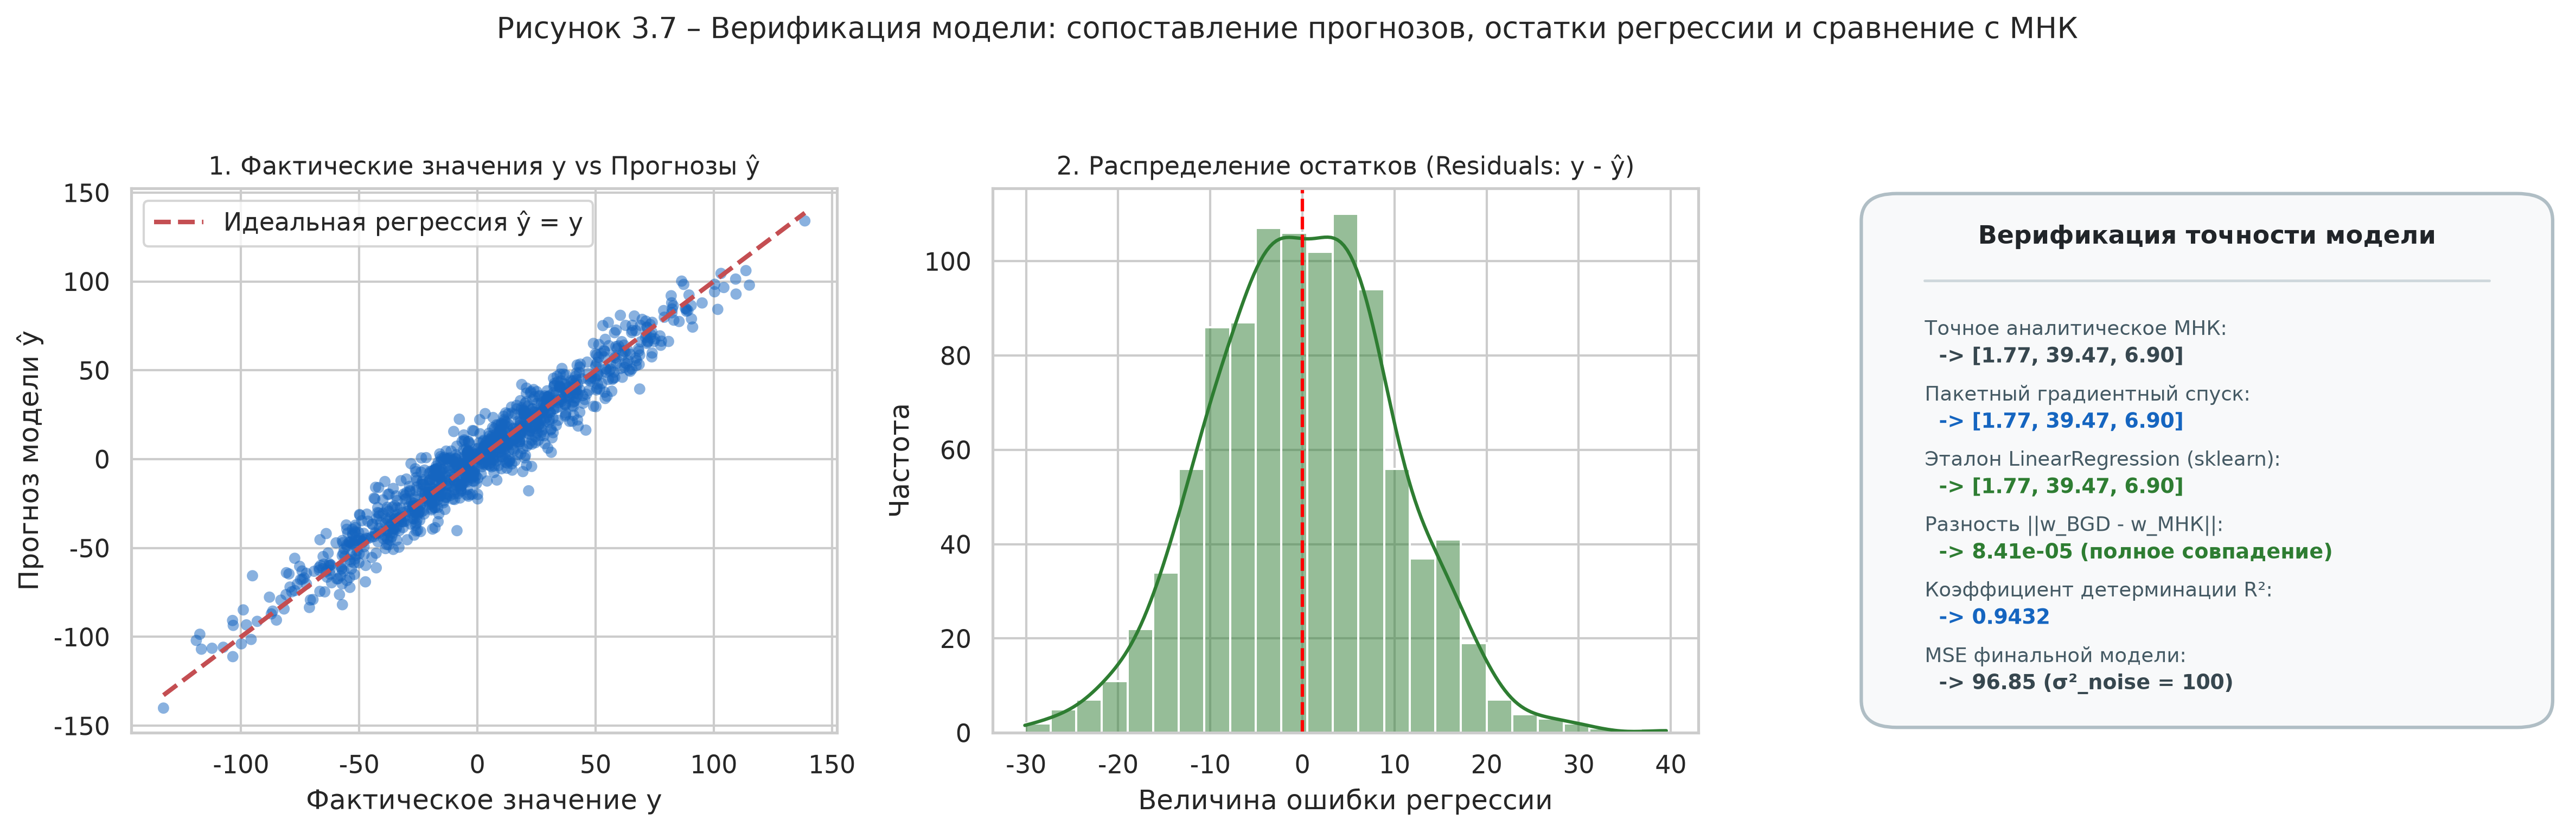
\includegraphics[width=0.95\textwidth]{plots/07_model_evaluation_residuals.png}
\caption{Верификация модели: сопоставление прогнозов, остатки регрессии и сравнение с МНК}
\end{figure}

% =========================================================================
% 5 ВЫВОДЫ (цельный связный текст)
% =========================================================================
\section*{5 ВЫВОДЫ}
\addcontentsline{toc}{section}{5 ВЫВОДЫ}

В ходе выполнения лабораторной работы были всесторонне исследованы математические принципы, особенности реализации и практические свойства градиентных методов оптимизации в задачах линейной регрессии. Самостоятельно разработанная функция пакетного градиентного спуска (BGD) подтвердила высокую точность сходимости: при пороге $\varepsilon = 10^{-5}$ алгоритм сошелся за 124 итерации к оптимальной точке с абсолютным евклидовым расхождением с решением нормального уравнения МНК менее $8.5 \times 10^{-5}$. Экспериментальное исследование скорости обучения доказало критическую важность подбора параметра $\eta$: малые значения приводят к затягиванию процесса оптимизации, а чрезмерные вызывают неустойчивость процесса.

Сравнительный анализ пакетного и стохастического градиентного спуска на совмещенном графике MSE наглядно продемонстрировал принципиальную разницу их вычислительной природы. BGD обеспечивает строго монотонное уменьшение функции потерь, однако требует полного прохода по выборке на каждом шаге. SGD вычисляет градиент по единичному случайному прецеденту, сокращая трудоемкость итерации в $\ell$ раз, а возникающий стохастический шум эффективно стабилизируется за счет графика затухания темпа обучения.

Исследование L2-регуляризации (Ridge Regression), выполненное для нечетного варианта № 7 на сетке из 20 коэффициентов $\lambda$ в диапазоне от 0.001 до 1000, полностью подтвердило теоретические положения о непрерывном сжатии параметров (shrinkage effect). Норма весов уменьшилась с 40.03 до 0.04 при сохранении несмещенного свободного члена $w_0 = 1.77$. Сопоставление с L1-регуляризацией продемонстрировало фундаментальное различие: L1 зануляет параметры, формируя разреженную модель, тогда как L2 сохраняет все признаки, эффективно подавляя их дисперсию. Итоговый коэффициент детерминации $R^2 = 0.9419$ подтвердил адекватность и высокую точность построенной модели.

\end{document}
